\begin{enumerate}[label=\thechapter.\arabic*,ref=\thechapter.\theenumi]

\item The number of zeroes of the polynomial $P(s) = s^3+2s^2+5s+80$ in the right side of the plane?\hfill(GATE IN 2023) \\

\solution
\iffalse
\let\negmedspace\undefined
\let\negthickspace\undefined
\documentclass[journal,12pt,twocolumn]{IEEEtran}
\usepackage{cite}
\usepackage{amsmath,amssymb,amsfonts,amsthm}
\usepackage{algorithmic}
\usepackage{graphicx}
\usepackage{textcomp}
\usepackage{xcolor}
\usepackage{txfonts}
\usepackage{listings}
\usepackage{enumitem}
\usepackage{mathtools}
\usepackage{gensymb}
\usepackage{comment}
\usepackage[breaklinks=true]{hyperref}
\usepackage{tkz-euclide} 
\usepackage{listings}
\usepackage{gvv} 
\usepackage{caption}
\def\inputGnumericTable{}                   

%\usepackage[latin1]{inputenc}                                
\usepackage{color}                                            
\usepackage{array}                                            
\usepackage{longtable}                                       
\usepackage{calc}                                             
\usepackage{multirow}                                         
\usepackage{hhline}                                           
\usepackage{ifthen}                                           
\usepackage{lscape}

\newtheorem{theorem}{Theorem}[section]
\newtheorem{problem}{Problem}
\newtheorem{proposition}{Proposition}[section]
\newtheorem{lemma}{Lemma}[section]
\newtheorem{corollary}[theorem]{Corollary}
\newtheorem{example}{Example}[section]
\newtheorem{definition}[problem]{Definition}
\newcommand{\BEQA}{\begin{eqnarray}}
\newcommand{\EEQA}{\end{eqnarray}}
\newcommand{\define}{\stackrel{\triangle}{=}}
\theoremstyle{remark}
\newtheorem{rem}{Remark}

\begin{document}

\bibliographystyle{IEEEtran}
\vspace{3cm}

\title{GATE: IN - 24.2023}
\author{EE23BTECH11013 - Avyaaz$^{*}$% <-this % stops a space 
}
\maketitle
\newpage
\bigskip

\renewcommand{\thefigure}{\arabic{figure}}
\renewcommand{\thetable}{\arabic{table}}

\large\textbf{\textsl{Question:}}
The number of zeroes of the polynomial $P(s) = s^3+2s^2+5s+80$ in the right side of the plane?\hfill(GATE IN 2023) \\
\solution
\fi
The table below shows the Routh array of the $n^{th}$- order characteristic polynomial : 
\begin{align}
    a_0s^n+a_1s^{n-1}......+a_{n-1}s^1+a_ns^0
\end{align}

\begin{table}[htbp]
\setlength{\extrarowheight}{8pt}
\centering
\begin{tabular}{|c|c|c|c|c|}
\hline 
$s^n$ & $ a_0 $ & $a_2 $ &  $a_4$ & ... \\
\hline
$s^{n-1}$ &$a_1$&$a_3$&$a_5$&...  \\
\hline
$s^{n-2} $& $b_1 = \dfrac{a_1a_2-a_3a_0}{a_1}$ &$b_2 = \dfrac{a_1a_4 - a_5a_0}{a_1}$ &...&..\\
\hline
$s^{n-3} $& $c_1 = \dfrac{b_1a_3-b_2a_1}{b_1}$  & $\vdots$ && \\
\hline
$\vdots$ & $\vdots$ & $\vdots$&&\\
\hline
$s^1$&$\vdots$&$\vdots$&&\\
\hline
$s^0$&$a_n$&&&\\
\hline
\end{tabular}

\caption{Routh Array}
\label{tab:routharray.IN.24.2023}
\end{table}
 Characteristic Equation:
\begin{align}
   s^3+2s^2+5s+80 = 0  
\end{align}


\noindent From \tabref{tab:routharray.IN.24.2023}:

\begin{table}[htbp]
\setlength{\extrarowheight}{10pt}
\centering
\begin{tabular}{|c|c|c|}
\hline 
$s^3$ & $ 1 $ & $5$ \\
\hline
$s^2$ &$2$&$80$ \\
\hline
$s^1 $& $\dfrac{2\times 5-80\times1}{2}= 
 -35$ & \\
\hline
$s^0 $& $ \dfrac{-35 \times 80}{-35} = 80$ &\\
\hline
\end{tabular}

\caption{}
\label{tab:inputs.IN.24.2023}
\end{table}

% The number of sign changes of the terms of the first column of the Routh Array corresponds to the number of roots of the characteristic equation in the right half of the s-plane.

\noindent From \tabref{tab:inputs.IN.24.2023}:

Since there are 2 sign changes in the first column of the Routh tabulation. So, the number of zeros in the right
half of the s-plane will be 2.

% s1 = -4.63925
% s2 = 1.31963 + 3.93735 i
% s3 = 1.31963 - 3.93735 i
% A pole is a value of s (in the Laplace domain) for which the transfer function becomes infinite.
% A zero is a value of s for which the transfer function becomes zero.

% In the Laplace domain, a transfer function 
% H(s) is typically represented as a ratio of polynomials in s: H(s)= N(s)/D(s)

\begin{figure}[htbp]
    \centering
    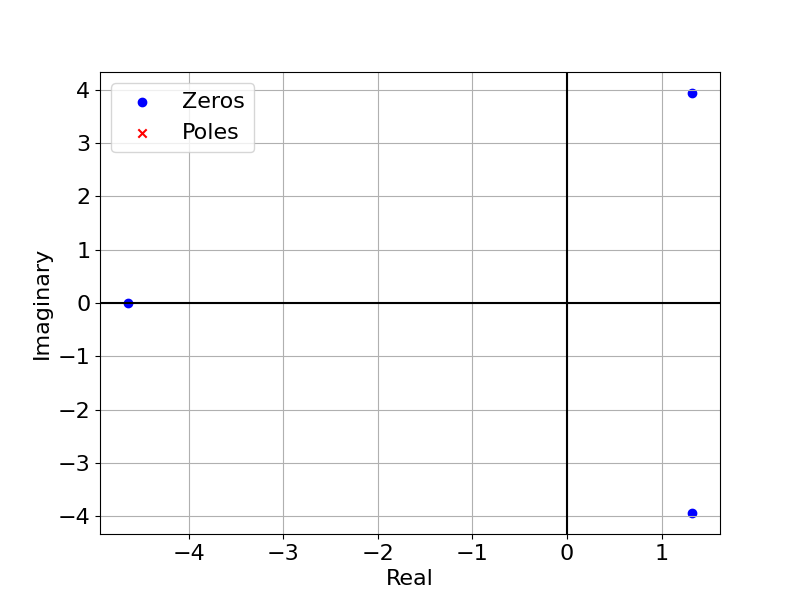
\includegraphics[width = \columnwidth]{2023/IN/24/figs/poles and root_plot.png}
  \caption{}
    \label{fig:graph1}
\end{figure}

% \bibliographystyle{IEEEtran}

\newpage

\item The circuit shown in the figure is initially in the steady state with the switch K in open condition and $\overline{K}$ in closed condition. The switch K is closed and $\overline{K}$ is opened simultaneously at the instant $t = t_1$, where $t_1 > 0$. The minimum value of $t_1$ in milliseconds such that there is no transient in the voltage across the 100 $\mu F$ capacitor, is \rule{1cm}{0.15mm} (Round off to 2 decimal places) \hfill (GATE EE 2023)
    \begin{circuitikz}[american]
        \draw (0,7) to [R=10$\Omega$] (0,2) to [short] (3.5,2) to [isource, l={$\sin\brak{1000t}$}] (3.5,7) to [short] (0,7);
        \draw (3.5,2) to [short] (5,2) to [short] (5,0) to [R=$10\Omega$] (7.5,0) to [battery2 = 5V] (10,0) to [short] (10,2) to [curved capacitor=100$\mu$F, invert] (10,7) to [short] (5,7) to [short] (3.5,7);
        \draw (5,2) to [short] (7, 2) to[ospst=$\overline{K}$] ++(1,0);
        \draw (5,5) to [short] (5,2);
        \draw (10,2) to [short] (8,2);
        \draw (5,7) to [short] (5,6) to[cspst=K] ++(0,-1) ;
\end{circuitikz}


\newpage

\end{enumerate}
